%!TEX encoding = UTF-8 Unicode
%!TEX root = ../lect-week14.tex

%%%

\Subsection{Tentatips}
\begin{Slide}{Före tentan:}\SlideFontSmall
\begin{enumerate}
\item Repetera övningar och labbar i kompendiet. 
\item Läs igenom föreläsningsanteckningar.
\item Studera \Emph{snabbref} \Alert{mycket noga} så att du vet vad som är givet och var det står, så att du kan hitta det du behöver snabbt.
\item Skapa och \Emph{memorera} en personlig \Emph{checklista} med programmeringsfel du brukar göra, som även inkluderar småfel, så som glömda parenteser och semikolon, och annat som en kompilator/IDE normalt hittar.
\item Tänk igenom hur du ska disponera dina 5 timmar på tentan.
\item Gör den minst en extenta som om det vore \Alert{skarpt läge}: 
\begin{enumerate}\SlideFontTiny
\item Avsätt 5 ostörda timmar (stäng av telefon, dator etc).
\item Inga hjälpmedel. Bara snabbref.
\item Förbered dryck och tilltugg.
\end{enumerate}
\end{enumerate}
\end{Slide}

\begin{Slide}{På tentan:} \SlideFontTiny
\begin{enumerate}
\item Läs igenom \Alert{hela} tentan först. \\ \Emph{Varför?} Förstå helheten. Delarna hänger ihop.
\item Notera och begrunda specifika begrepp och definitioner. \\ \Emph{Varför?} Begreppen är avgörande för förståelsen av uppgiften.
\item Notera förenklingar, antaganden och specialfall. \\ \Emph{Varför?} Uppgiften blir mkt enklare om du inte behöver hantera dessa.
\item \Alert{Fråga} tentamensansvarig om du inte förstår uppgiften -- speciellt om det finns misstänkta felaktigheter eller förmodat oavsiktliga oklarheter. \\ \Emph{Varför?} Det är inte lätt att konstruera en ''perfekt'' tenta. \\ Du får fråga vad du vill, men det är inte säkert du får svar :)
\item Läs specifikationskommentarerna och metodsignaturerna i alla givna klass-specifikationer \Alert{mycket noga}. \\ \Emph{Varför?} Det är ett vanligt misstag att förbise de ledtrådar som ges där.
\item Återskapa din memorerade personliga checklista för vanliga fel som du brukar göra och avsätt tid till att gå igenom den på tentan. Varje fix plockar poäng!
\item Lämna in ett försök även om du vet att lösningen inte är fullständig. Det gäller att ''plocka poäng'' på så mycket som möjligt. En dålig lösning kan ändå ge poäng.

\item Om du har svårigheter kan det bli kamp mot klockan. Försök hålla huvudet kallt och prioritera utifrån var du kan plocka flest poäng. Ge inte upp! Ta en kort äta-dricka-paus för att få mer energi!

\end{enumerate}
\end{Slide}

\ifkompendium\else

\begin{Slide}{Planeringstips}\SlideFontTiny
Exempel på saker som du kan lägga in tid för i din julpluggkalender:
\begin{enumerate}
\item Välja ut övningar att repetera
\item Repetera övning X, Y, Z, ... Både läsa och skriva kod. Fundera på typ och värde.
\item Välja ut labbar att repetera
\item Repetera labb X, Y, Z, ... Lär dig ''trick'' och ''mönster''.
\item Träna på att skriva program med papper och penna
\item Göra checklista med vanliga fel
\item Läsa igenom extentor i Java
\item Välja ut minst en Java-extenta att göra som i skarpt läge i Scala
\item Gör Java-extentor X, Y, Z, ... implementera (delar) i Scala
\item Gör utvalda delar av extenta X, Y, Z, ... i Java
\end{enumerate}
\end{Slide}

\Subsection{Avgränsning}

\begin{Slide}{Tentans struktur}
\begin{itemize}
\item Del A 20\%:\\\Emph{Läsa uttryck} där du ska \Alert{ange typ och värde}
\begin{itemize}\SlideFontTiny
\item Du kommer att behöva skriva ner delsteg och variablers värden (minnet)
\item Testar förståelse av variabler, uttryck, samlingar, algoritmer, arv, etc.
\item Uppdaterad (mildare) regel om ''rättningströskel'': \\
Ur senaste compendium.pdf kapitel 0.8: \textit{Om du på del A erhåller färre poäng än vad som krävs för att nå upp till en bestämd ''rättningströskel'', kan din tentamen komma att underkännas utan att del B bedöms.}
\item Liknar kompendiets övningar; rimlig att lösa och dubbelkolla på 1h
\end{itemize}


\item Del B 80\%:\\\Emph{Skriva kod} som uppfyller \Alert{krav och designspecifikation}
\begin{itemize}\SlideFontTiny
\item Testar att du själv kan skapa kod med delar som samverkar
\item Testar förmåga att gå från indata-utdata till algoritm \\
 givet: ledtrådar, design, ev. skiss på lösning, ev. pseudokod etc.
\item Liknar kompendiets labbar; rimlig att lösa och dubbelkolla på 4h 
\end{itemize}

\end{itemize}
\end{Slide}



\begin{Slide}{Vad kommer på tentan? (1 av 3)}\SlideFontTiny
\hspace{-1em}\begin{minipage}{1.0\textwidth}
Allmänt: 
\begin{itemize}\SlideFontTiny
\item Begrepp som är ''fördjupning'' krävs ej på tentan (men ökar förståelse)
\item Ok om du väljer en enklare lösning med basala begrepp som fungerar bra, \\i stället för en kortare/elegantare/mer avancerad lösning
\item Dessa moduler ingår ej på tentan: ''Trådar, webb'', ''Design, api''
\end{itemize}

\vspace{1em}\begin{tabular}{l | l | l}
\textbf{Modul} & \textit{Ingår t.ex.}& \textit{Avgränsning} (ej krav; ok anv. om lämpl.)\\\hline
Introduktion & uttryck, aritmetik, slumptal, & kan ha nytta av deMorgan men ej krav\\
             & strängar, typer, Unit   & skriva egna \code|s"$x"| (men kunna läsa)  \\
             & skillnad mellan heltal \& flyttal & Float, Byte, Short\\
             & variabler, for, while, if & hex-literaler, backticks\\ 
\hline
Kodstrukturer & iterering, SWAP, SUM, MIN/MAX & import, paketnamn\\             
              & loopar, Range, sats vs uttryck & ok att välja vilken loop du tycker passar\\
              & namn, synlighet, skuggning & scaladoc, javadoc, jar \\        
\hline
Funktioner,   & definiera, anropa, parameter& skapa egen kontrollstruktur\\
objekt        & returtyp, namnarop, defaultarg & stegad funktion, rekursion\\        
              & punktnotation, objekt vs static & lazy val\\        
              & map/foreach med egen funktion & \\
              & anonyma funktioner (lambda)  & \\                              

\end{tabular}
\end{minipage}
\end{Slide}


\begin{Slide}{Vad kommer på tentan? (2 av 3)}\SlideFontTiny
\hspace{-2em}\begin{minipage}{1.0\textwidth}
\begin{tabular}{l | l | l}
\textbf{Modul} & \textit{Ingår t.ex.}& \textit{Avgränsning} (ej krav; ok anv. om lämpl.)\\\hline
Datastrukt. & attribut, medlem, metod, klass & isInstanceOf (anv. match istället) \\
            & tupler, Vector, Set, Map & List (oftast Vector istället)\\
            & Source.fromFile          & java.nio.file \\
\hline
Sekvensalg. &  skapa ny samling från befintlig &  \\      
            &  registrering, Scanner, ArrayBuffer & StringBuilder\\
            &  uppdatera Array, ArrayBuffer, Vector & \\
            &  slumptalsfrö, scala.util.Random  &  \\
\hline

Klasser     &  new, this, synlighet  & null \\
            &  inkapsling, accessregler, private  & private[this] \\
            &  klassparameter, fabriksmetod  & \\
            &  class vs case class    & \\
            &  referenslikhet vs innehållslikhet    & \\
            &  föränderlig vs oföränderlig klass & \\
\hline
Arv         &  bastyp, subtyp, trait, extends  & \\
            &  överskuggning,                  & inmixning, \\
            &  Any, AnyVal, AnyRef, Object     & Null, Nothing\\
            &  accessregler vid arv, protected & final\\
            &  abstract class, case object     & \\
            
\end{tabular}
\end{minipage}
\end{Slide}


\begin{Slide}{Vad kommer på tentan? (3 av 3)}\SlideFontTiny
\hspace{-2em}\begin{minipage}{1.0\textwidth}
\begin{tabular}{l | l | l}
\textbf{Modul} & \textit{Ingår t.ex.}& \textit{Avgränsning} (ej krav; ok anv. om lämpl.)\\\hline

Mönster     & match, Option, Try & try catch, unapply\\
            & flatten, sealed            & flatMap, partiella funktioner\\
            & enkel equals utan arv     & hashcode, fullständig equals   \\ 
            & wildcard-mönster  & variabelbindn. i mönster, sekvensmönster\\
\hline

Matriser,     & indexering i nästlade strukturer & \\
typparametrar & nästlad for-sats  & \\ 
              & matriser i Java med array  & \\
              & använda generiska strukturer & skapa generiska strukturer\\ 
\hline

Sök, sortera & linjärsökning, binärsökning & algoritmisk komplexitet\\
            & compareTo, strängjämförelse & Ordering, Ordered\\
            & insättningssortering & räcker kunna en valfri sortering \\
\hline


Scala/Java & översätta enkel Java/Scala & try catch i Java \\
           & implemenetera Java-klass     &  arv i Java med super vid konstr.\\
           & grundläggande syntaxskillnader & \\
           & ArrayList vs ArrayBuffer & java.util.\{List, Set\}\\
           & Autoboxing vid ArrayList<Integer> & \\
\multicolumn{3}{c}{OBS! Java-övningar finns även här och där i andra moduler}\\
\hline           
     
\end{tabular}
\end{minipage}
\end{Slide}


\Subsection{Tips vid val av lösningar}


\begin{Slide}{Tips om val av klass/trait}\SlideFontSmall
Ofta ger tentan en specifik design, men du kan ha stor nytta av egna abstraktioner, speciellt \Emph{lokala funktioner} för att göra enklare dellösningar!

\pause\vspace{1em}Om du skulle behöva samla både attribut och metoder utöver givna specifikationer:
Singelobjekt, case-klass, klass, trait eller abstrakt klass?
\begin{itemize}\SlideFontTiny
\item Använd \code{object} om du behöver samla metoder (och variabler) i en modul som bara finns i en upplaga. Du får lokal namnrymd och punktnotation på köpet.
\item Använd en \code{case class} om du har \Emph{oföränderlig data}. Du får då även innehållslikhet, möjlighet till mönstermatchning, etc. på köpet! 
\item Behöver du \Alert{föränderligt tillstånd} använd en vanlig \code{class}.\\ Det normala är att tillståndet (alla attribut) är \code{private} eller \code{protected} och att all uppdatering och avläsning av tillståndet sker indirekt genom metoder (getters/setters/...). 
\item Behöver du en abstrakt bastyp utan konstruktorparametrar använd en \code{trait}. \\(Du får inmixningsmöjlighet med \code{with} på köpet. Inmixning kommer ej på tenta.)
\item Behöver du en abstrakt bastyp med konstruktorparametrar använd en \code{abstract class}. (Går dock ej att använda vid inmixning med \code{with}.)
\end{itemize}
\end{Slide}


\begin{Slide}{Tips om hur man läser en specifikation}\SlideFontSmall
När du läser en specifikation av en klass, en trait, eller ett singelobjekt:
\begin{itemize}
\item Tänk igenom vilket ansvar olika delar av koden har
\item Vad håller klassen reda på? \\$\rightarrow$ Ledtrådar till attribut
\item Vad ska klassen göra/räkna ut? \\$\rightarrow$ Ledtrådar till metoder och deras algoritm
\item Vilka andra klasser har nytta av denna metod? \\$\rightarrow$ Ledtrådar till hur klasserna samverkar för att lösa uppgiften
\end{itemize}
Rita gärna en bild med ett specifikt exempel på vilken data som olika instanser håller reda på och fundera på hur data skapas/beräknas/förändras
\end{Slide}


\begin{Slide}{Tips om val av samling}\SlideFontSmall

Generellt: Det är ofta enklare med oföränderliga samlingar med oföränderliga element och skapa nya samlingar vid förändring. Men ibland blir det enklare om man har föränderliga samlingar.

\begin{itemize}
\item Behöver du hantera värden \code{x} av t.ex. typen String med \Emph{heltalsindex}?
\begin{itemize}\SlideFontTiny
\item Om du klarar dig utan förändring av innehållet:\\ \code{ val xs: Vector[String]}
\item Om du behöver ändra innehåll men \Alert{inte} antal element: \\ \code{ val xs: Array[String]} 
\item Om du behöver ändra innehåll \Alert{och} antal element: 
\\ \code{ var xs: Vector[String] } (se metoden \code{patch}) eller \\ \code{ val xs: ArrayBuffer[String]} (har metoden \code{insert})
\end{itemize}

\item Behöver du hantera värden \code{x} som ska vara unika?
\begin{itemize}\SlideFontTiny
\item Oföränderlig: \code{  val xs: Set[String] }
\item Förändringsbar: \code{val xs: scala.collection.mutable.Set[String]}
\end{itemize}

\item Behöver du leta upp värden \code{x:Int} utifrån en nyckel av t.ex. String?
\begin{itemize}\SlideFontTiny
\item Oföränderlig: \code{   val xs: Map[String, Int] }
\item Förändringsbar: \code{val xs: scala.collection.mutable.Map[String, Int]}
\end{itemize}


\end{itemize}
\end{Slide}

\begin{Slide}{Tillåtna uppdateringar i din QuickRef}
Du får med egen penna göra dessa fixar i din QuickRef:
\begin{itemize}
\item Grundtypernas implementation, sid 4: 
\begin{itemize}

\item omfång för Int ska ha exponent 31 (inte 15), 
\item omfång för Long ska ha exponent 63 (inte 15).
\end{itemize}

\item Saknade samlingsmetoder: 
\begin{itemize}
\item Under rubriken "Methods in trait Map[K, V]" saknas metoderna keySet och mapValues. 
\item Saknade metoderna för mutable.ArrayBuffer[T]: \\ \code{update} \code{insert} \code{remove} \code{append} \code{prepend}, etc. \\ lägg till beskrivning på lediga platsen på sista sidan \\ 
(se vidare commit \href{https://github.com/lunduniversity/introprog/commit/a5e29d000062}{a5e29d000062a} i kursrepot)
\end{itemize}
\end{itemize}
\end{Slide}


\begin{Slide}{ArrayBuffer}
Viktigast att känna till: update, insert, remove, append
{\SlideFontTiny

\vspace{2.5em}\begin{tabular}{@{}p{4.2cm}  p{6.5cm}}
\texttt{xs(i) = x \newline xs.update(i, x)} & Replace element at index i with x. \newline Return type Unit.\\   \cline{1-2}

\texttt{xs.insert(i, x)\newline xs.remove(i)} & Insert x at index \texttt{i}. Remove element at i. \newline Return type Unit.\\   \cline{1-2}

\texttt{xs.append(x)~~~xs~+=~x} & Insert x at end.  Return type Unit.\\   \cline{1-2}

\texttt{xs.prepend(x)~~x~+=:~xs} & Insert x in front.  Return type Unit.\\   \cline{1-2}

\texttt{xs -= x} & Remove first occurance of x (if exists). \newline Returns xs itself. \\\cline{1-2}

\texttt{xs ++= ys} & Appends all elements in ys to xs and returns xs itself. \\

\end{tabular}
}
\end{Slide}



\Subsection{Genomgång av extenta}
\begin{Slide}{Extenta 2016-08-24 TimePlanner}\SlideFontSmall
\url{http://cs.lth.se/pgk/examination/}

\vspace{1em}\Alert{TimePlanner}: 
\begin{itemize}
\item \href{http://fileadmin.cs.lth.se/cs//Education/grundkurs/extentor/160824.pdf}{tentamen 160824} 
\item \href{http://fileadmin.cs.lth.se/cs//Education/grundkurs/extentor/sol-160824.pdf}{lösningsförslag Java} 
\item \href{https://github.com/lunduniversity/introprog/tree/master/compendium/examples/exam/re-impl-java-exams/timeplanner-160824}{översättning av lösning till Scala}
\end{itemize}
\end{Slide}


\Subsection{Avslutning av kursen}

\begin{Slide}{Obligatoriska moment}\SlideFontSmall
\begin{itemize}
\item Kolla vilka oblikatoriska moment du har kvar här:
\url{http://fileadmin.cs.lth.se/pgk/SAM-EDAA45-snapshot.html}
\item Sök på din födelsemånad/dag, tex 0102 för andra januari.
\item Läs \Alert{alla} instruktioner \Alert{noga} och \Alert{anmäl dig} här: \\
\href{http://www.student.lth.se/studieinformation/anonyma-tentor/}{www.student.lth.se/studieinformation/anonyma-tentor}
\item Du ska vara godkänd på alla labbar+projekt för att få tenta pgk EDAA45!
\item Du ska vara godkänd på alla labbar+projekt för att få gå pfk \href{http://cs.lth.se/edaa01vt}{EDAA01}!
\item Använd återstående \Emph{resurstider} för \Alert{redovisning av labbar/projekt}.
\end{itemize}
\end{Slide}

\begin{Slide}{CEQ -- Course Experience Questionnaire}\SlideFontSmall
\begin{itemize}
\item Görs på hela LTH på samma sätt. Alla får länkar via mejl.
\item Snälla fyll i CEQ! Jag är \Alert{mycket tacksam} för all konstruktiv feedback! \\ Hög svarsfrekvens är viktigt för att kunna dra slutsatser om variationen i svaren och signifikansen i sammanställningen.
\item Del 1: Generella påståenden, alla med 5-gradig skala: \\ tar helt avstånd ... instämmer helt
\item Del 2: \Emph{Fritextfrågor}: \\
''Vad  tycker  du  var  det  bästa  med  den här  kursen?'' \\
''Vad  tycker  du  främst  behöver  förbättras?''
\item Fördel med CEQ: Samma alla kurser alla år medger jämförelse över tid.
\item Begränsning med CEQ: Saknar frågor kopplat till specifika kursmoment.
\item Mer om CEQ här: \url{https://www.ceq.lth.se/}
\end{itemize}
\end{Slide}

\begin{Slide}{Kursspecifik utvärdering om specifika kursmoment}\SlideFontSmall
\begin{itemize}
\item Jag vill gärna att alla gör den LTH-gemensamma, anonyma kursutvärderingsenkäten \href{https://www.ceq.lth.se/}{CEQ}. Dina fritext-kommentarer om vad som är det bästa med kursen och vad som främst behöver förbättra emottages mycket tacksamt i CEQ-utvärderingen!
\item Jag kommer att komplettera CEQ med en \Emph{kursspecifik} utvärdering av specifika kursmoment i denna kurs och jag är därför \Alert{mycket tacksam} om alla fyller enkäten när länk kommer via mejl. 
\item Jag behandlar dina svar konfidentiellt, men ber om din STiL-id så att jag kan återkomma om jag mot förmodan undrar något mer.
\item Din input är mycket värdefull vid framtida kursutveckling!
\end{itemize}
\end{Slide}

\begin{Slide}{Intresserad av att arbeta som handledare?}\SlideFontSmall
\begin{itemize}
\item 
\end{itemize}
\end{Slide}

\begin{Slide}{Utblick}\SlideFontSmall
Framtiden för \Emph{Scala}:
\begin{itemize}
\item Scala 2.12 bättre bytekod, Scala 2.13 bättre standardbibliotek
\item dotty och tasty
\item Scala.JS: dela kod+kompetens mellan backend och frontend
\item Scala native: kör Scala kompilerat direkt ''på metallen''
\end{itemize}
Några framtida \Emph{kurser} som direkt bygger på pgk:
\begin{itemize}
\item Fördjupningskursen (Java)
\item Utvärdering av programvarusystem (R)
\item Diskreta strukturer (Clojure)
\item Programvaruutveckling i grupp 
\item Objekt-orienterad modellering och design
\item Funktionsprogrammering 
\end{itemize}

\end{Slide}


\begin{Slide}{Hoppas att kursen varit kul och lärorik!}

\includegraphics[width=5cm]{../img/gurka.jpg}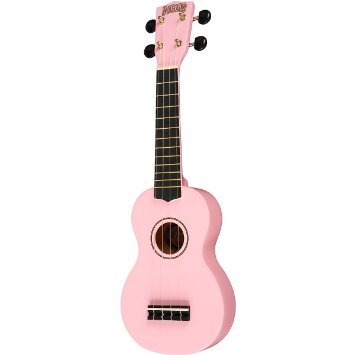
\includegraphics[width=5cm]{../img/ukulele.jpg}
\end{Slide}

\begin{Slide}{Ett stort TACK för...}
\begin{itemize}
\item ... att ni kämpat så hårt!
\item ... att ni ställt massor med frågor!
\item ... att det har varit så hög närvaro på föreläsningarna!
\item ... att ni är så konstruktiva och verkligen vill lära er!
\end{itemize}
\vspace{2em} \pause

\Alert{Ett stort LYCKA TILL på vägen till att bli en \\ kompetent och innovativ systemutvecklare!}
\end{Slide}


\fi